\chapter{Conclusions}

\begin{figure}[htp]
\begin{center}
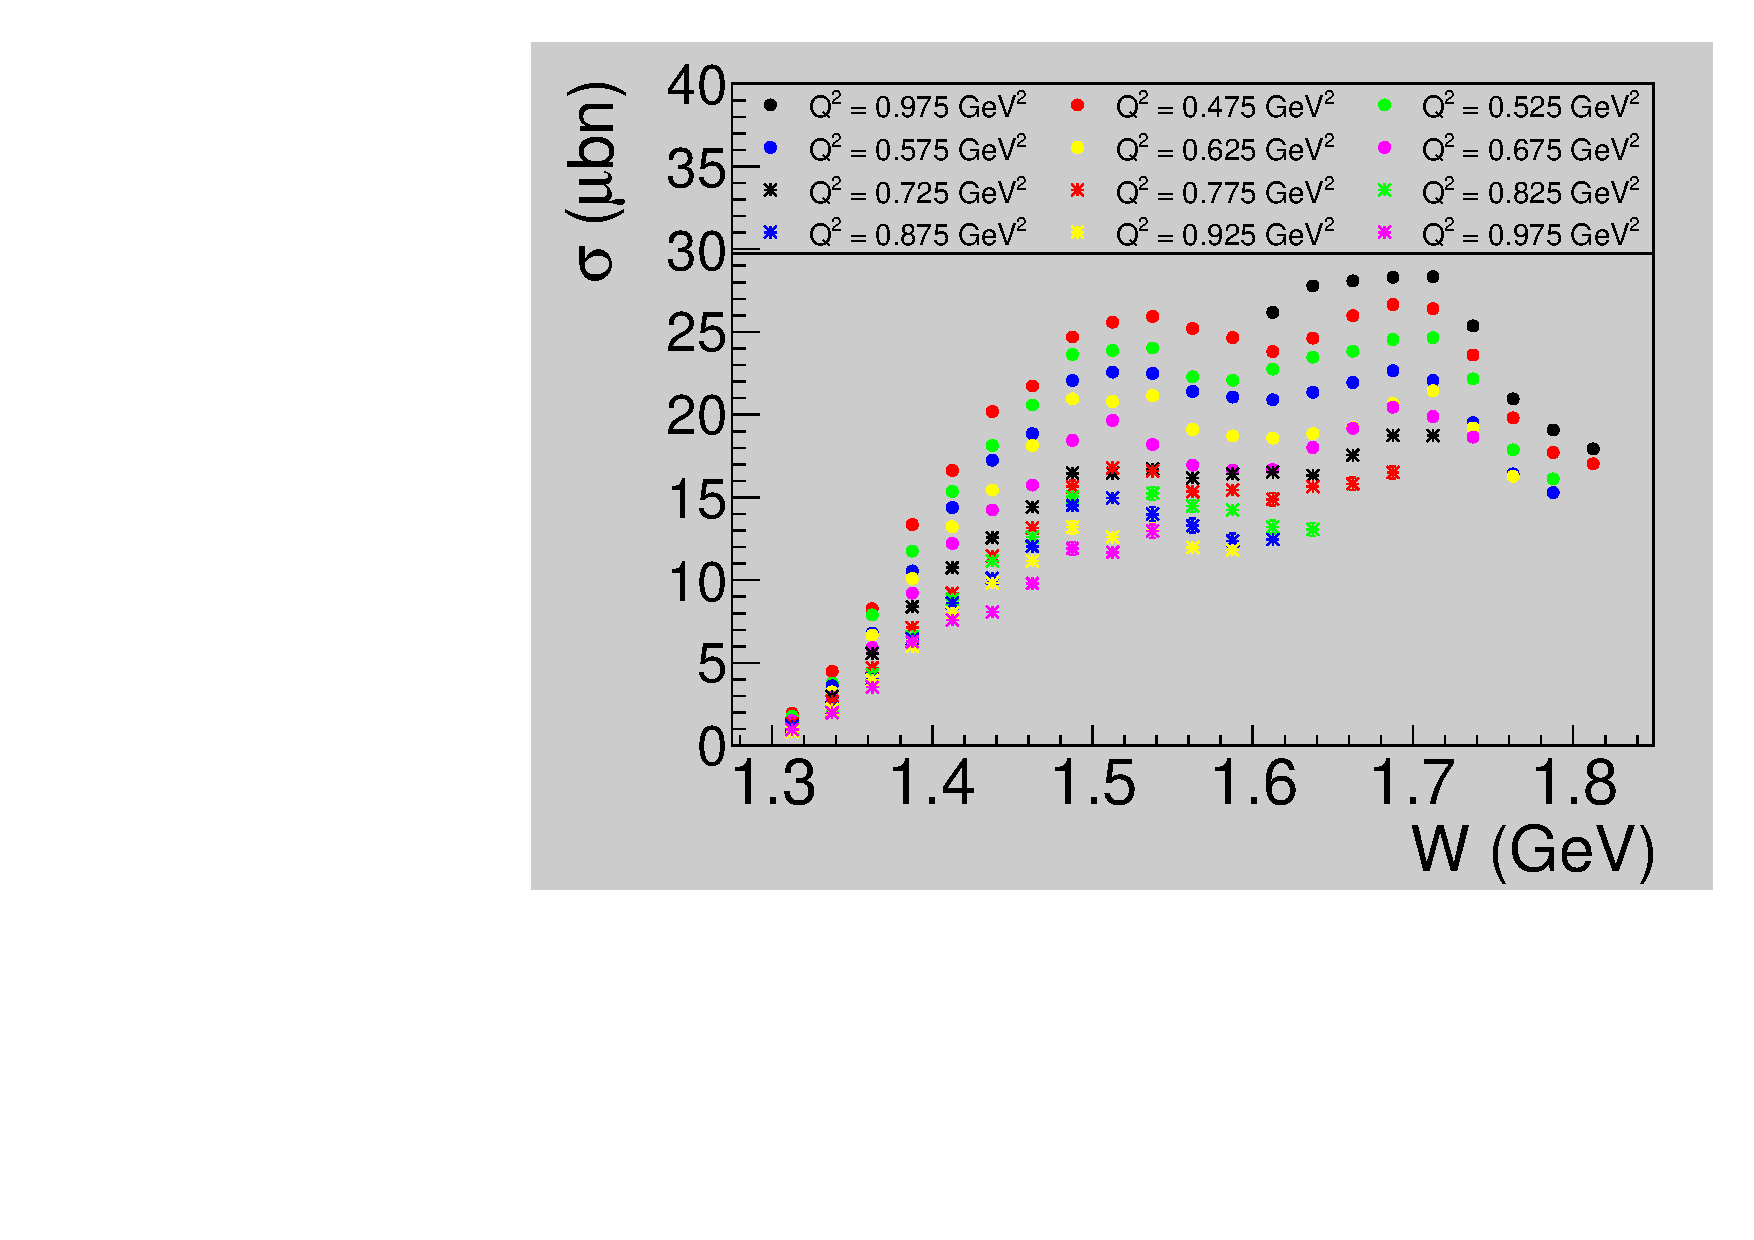
\includegraphics[width=12cm]{pictures/sys_err/all_q2.pdf}
\caption{\small $W$ dependencies of the integrated cross sections for various bins in $Q^{2}$}
\label{fig:all_q2}
\end{center}
\end{figure}


\begin{figure}[htp]
\begin{center}
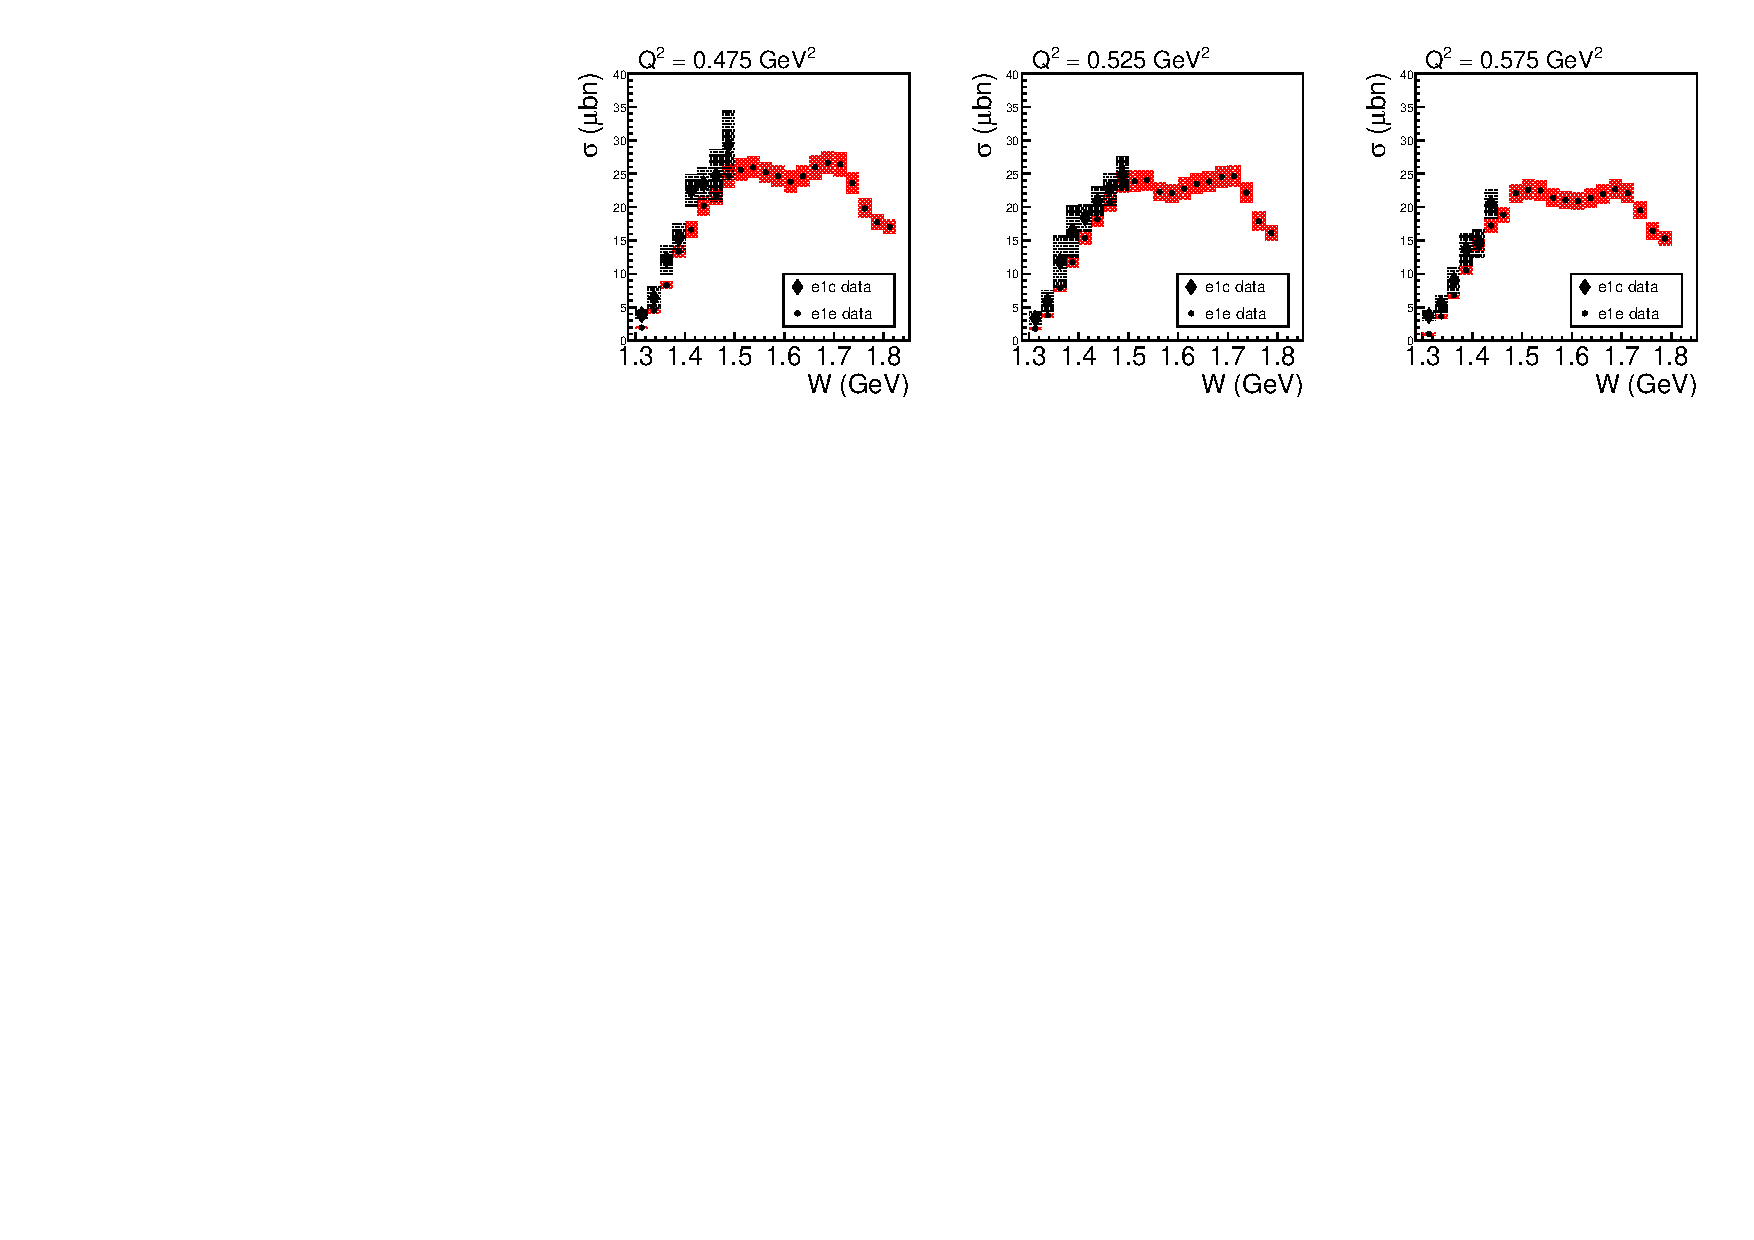
\includegraphics[width=12cm]{pictures/conclusions/e1e_e1c.pdf}
\caption{\small $W$ dependencies of the obtained in this analysis  cross sections (e1e dataset) in comparison with the cross sections from~\cite{Fedotov:2008aa} (e1c dataset) for three bins in $Q^{2}$. Hatched areas correspond to the total uncertainties (sistematical and statistical).}
\label{fig:e1e_e1c}
\end{center}
\end{figure}


\begin{itemize}

\item The complete set of the single-differential (see appendix~\ref{app_a}) and integrated cross sections (see Fig.~\ref{fig:all_q2}) for the reaction $\gamma_{v} p \rightarrow p \pi^{+} \pi^{-}$ is obtained in the range of $W$ from 1.3~GeV to 1.825~GeV and $Q^{2}$ from 0.45~GeV$^2$ to 1~GeV$^2$. The $Q^{2}$ binning of the cross sections in the kinematical area of high-lying nucleon resonances is six times finer than in previously avaliable data. 

\item The comparison of the obtained cross sections with the avaliable ones~\cite{Fedotov:2008aa} shows the reasonable agreement within the statistical uncertanties (see Fig.~\ref{fig:e1e_e1c}). It needs to be mentioned that this comparison is not fully justified since the cross sections from~\cite{Fedotov:2008aa} and this analysis are obtained with different beam energies.


\item The fit of these data by the meson-baryon reaction model JM~\cite{Mokeev:2008iw,Mokeev:2012vsa,Mokeev:2015lda} will provide for the first time information on the $Q^{2}$ evolution of high-lying resonances with very detailed binning.



\end{itemize}
